\headline{{\textbf{\Large\sffamily Club Exhibitions:}}\\
          {\textbf{\large\sffamily TWBC Winter Show}}}
\label{2025-01-winter}
\noindent
Join Us at the TWBC Winter Show 2025!

The Twickenham Bonsai Club (TWBC) is thrilled to announce the \textbf{TWBC Winter Show}, the first of our three annual bonsai shows and exhibitions. 
This highly anticipated event will take place on \textbf{Sunday, 2nd January 2025}, at \textbf{St Richard Reynolds Catholic College, Clifden Road, Twickenham, London, TW1 4LT}, from \textbf{10am to 4pm}. 
Whether you are a seasoned enthusiast or simply curious about bonsai, this promises to be a memorable day celebrating the artistry, dedication, and passion behind this living art form.

The Winter Show will feature around \textbf{fifty exquisite bonsai specimens,} including \emph{two trees that were part of the Federation of British Bonsai Societies' gold\--winning stand at Chelsea Flower Show}. These have been carefully selected to showcase a diverse range of styles, techniques, and species. Alongside these remarkable trees, we are delighted to include \textbf{suiseki tables,} celebrating the subtle beauty of stone appreciation—a perfect complement to the natural elegance of bonsai. Additionally, three bonsai traders will be present, offering pots, trees, and everything a bonsai enthusiast or beginner could need.

To make the day enjoyable and engaging for everyone, we have planned a variety of activities, including \textbf{interactive demonstrations,} and an \textbf{exhibition tour} to deepen your appreciation of the bonsai on display. For a touch of fun, don't miss our \textbf{tombola}, which offers the chance to win bonsai\--related prizes and other surprises. There truly is something for everyone!

\topic{A Club Effort}
\noindent
The TWBC Winter Show is a testament to the hard work and enthusiasm of our members and supporters, and we would like to express our heartfelt thanks to everyone who has contributed.

\begin{window}[%
    2,l,%
    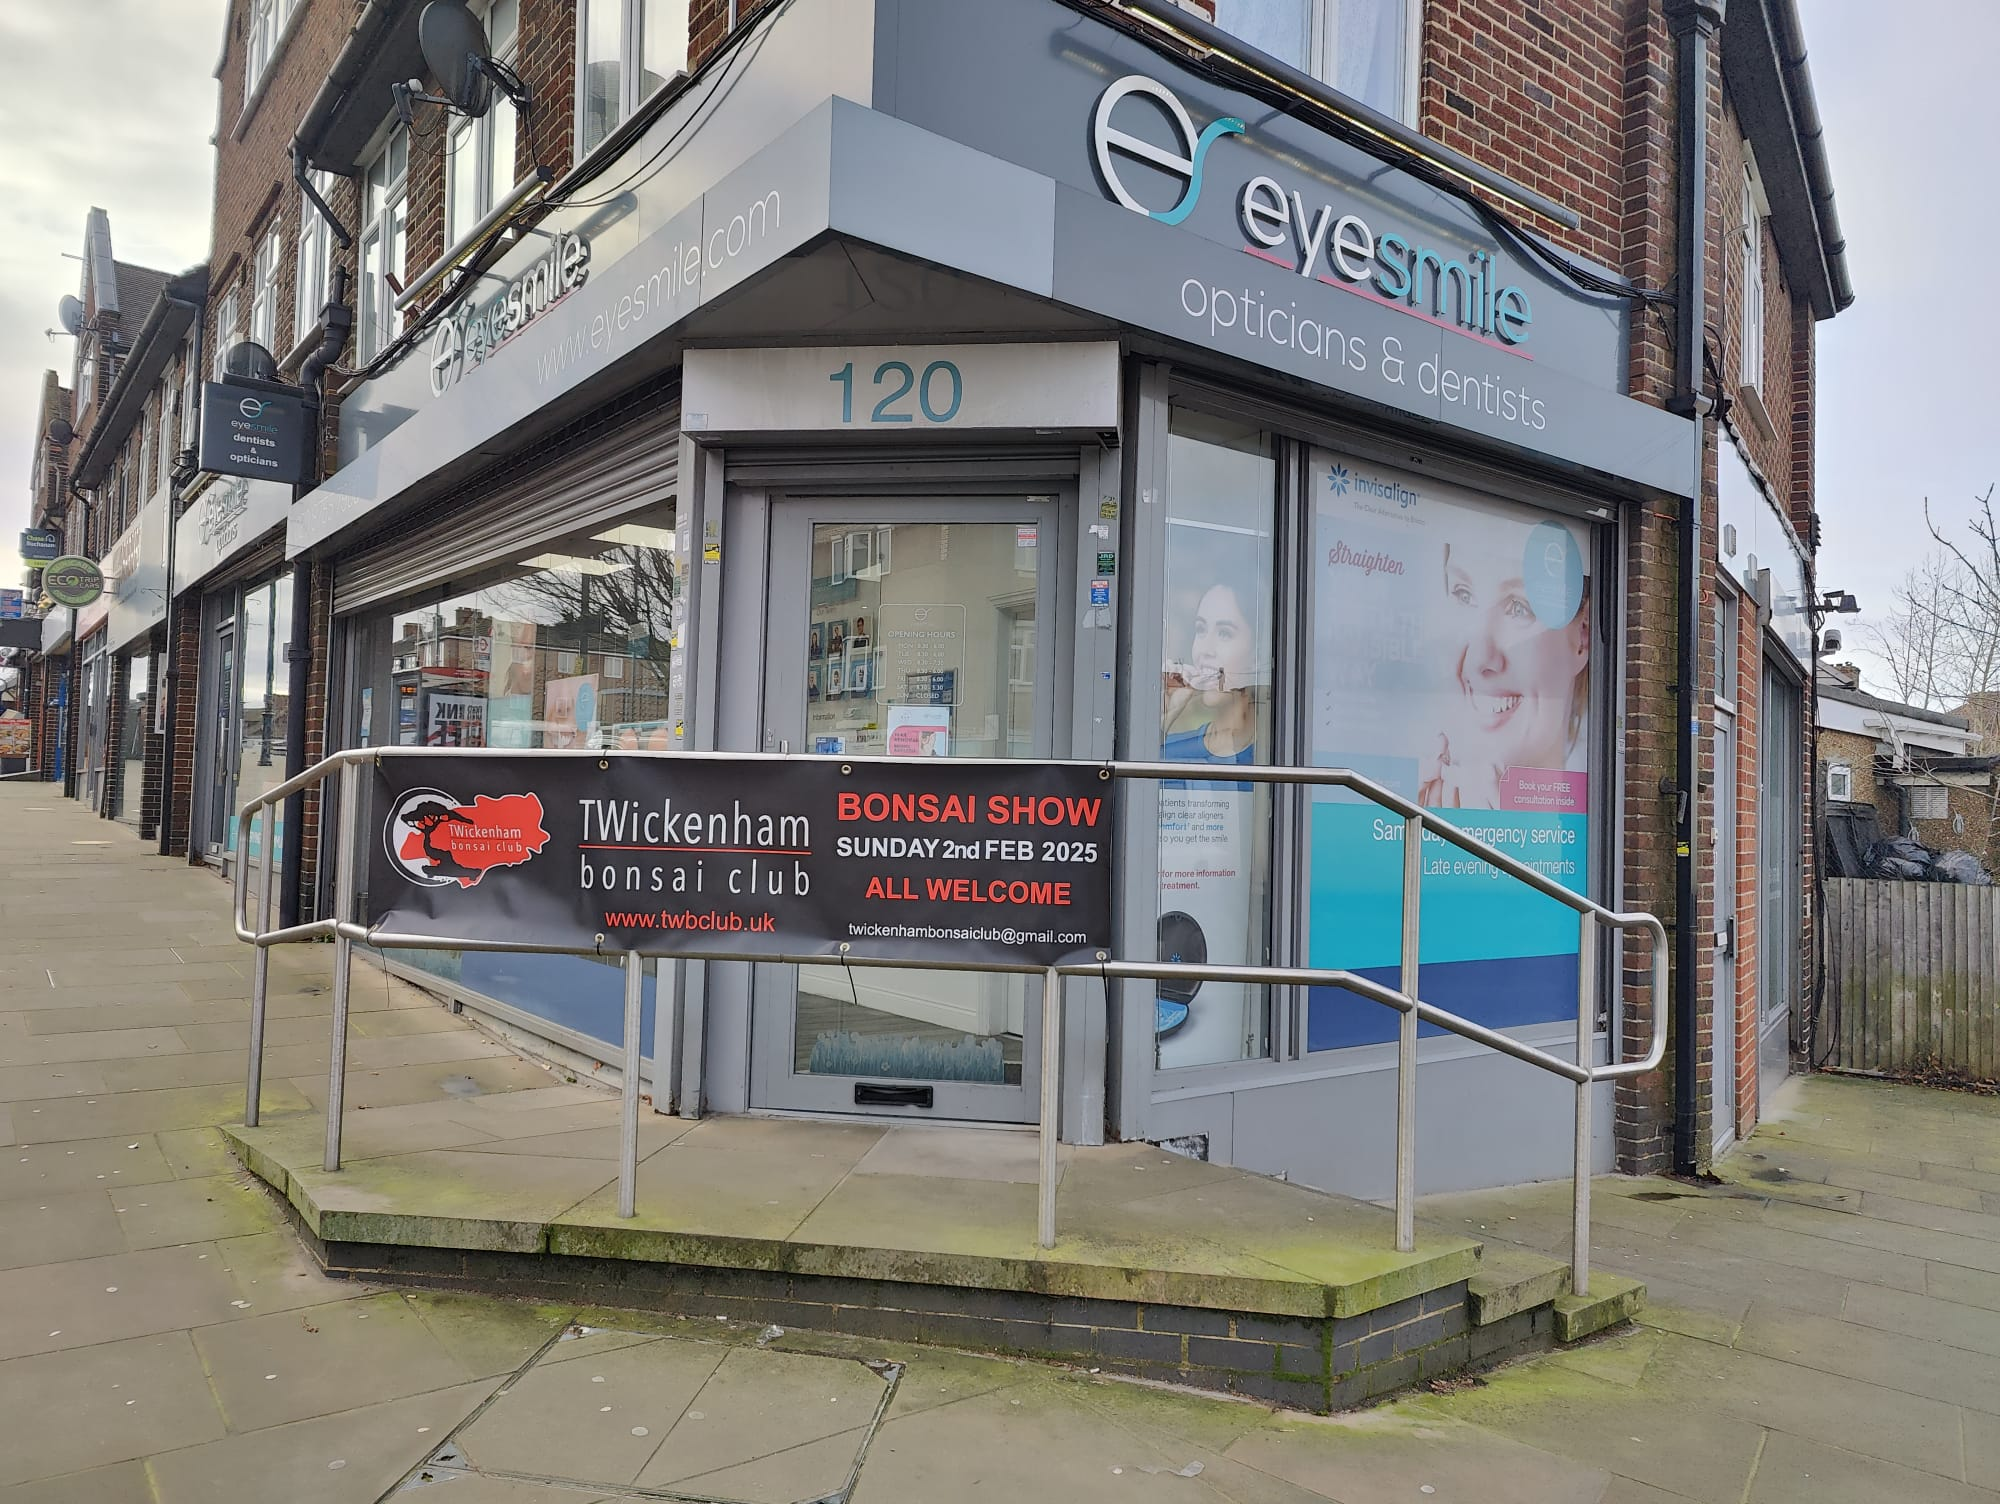
\includegraphics[width=1.0\columnwidth]{2025_01/res/show_sign.jpg},%
    \centerline{\emph{The TWBC Winter Show sign on display at EyeSmile}}\\%
    \centerline{\emph{in Whitton—our heartfelt thanks to them for their support!}}%
]
\end{window}
\columnbreak

\begin{itemize}
	\item \textbf{To those who helped put up street signs} to guide visitors: your efforts ensure we can welcome as many people as possible to share in our love of bonsai.
	
	\item \textbf{To everyone who submitted trees for consideration:} thank you for your dedication to nurturing these stunning specimens.
	
	\item \textbf{To the team who selected the bonsai for display:} your expertise ensures the exhibition represents the best of our club's talent.
	
	\item \textbf{To those supporting our suiseki tables:} thank you for highlighting this fascinating art form and enriching the experience for our attendees.
		
	\item \textbf{To the volunteers who have offered to help run the demonstrations and the tombola:} your commitment will ensure that attendees have an engaging and enriching experience throughout the day.
	
	\item \textbf{To those who will assist with setting up tables, arranging displays, and organising on the day of the event:} your support will be essential in creating a welcoming and well\--coordinated environment for everyone.
\end{itemize}

This is truly a team effort, and we hope to see many more members on the day to lend a hand. 
Whether it's helping with the setup, running activities, or simply greeting guests, every bit of support counts. 
Please arrive as early as possible to assist in creating a warm and welcoming atmosphere for everyone attending.

\topic{Spreading the Passion}
\noindent
Our goal is not only to showcase the beauty of bonsai but also to share the joy and dedication that go into cultivating these living masterpieces.
By hosting events like the Winter Show, we hope to inspire new enthusiasts and foster a deeper appreciation for bonsai in our community.

So, bring your friends, family, and curiosity to the TWBC Winter Show.
Let's make this a day to remember, filled with inspiration, learning, and connection.
Together, we can ensure the passion for bonsai continues to thrive.

We look forward to seeing you there!
\closearticle

\vfill
\begin{center}
	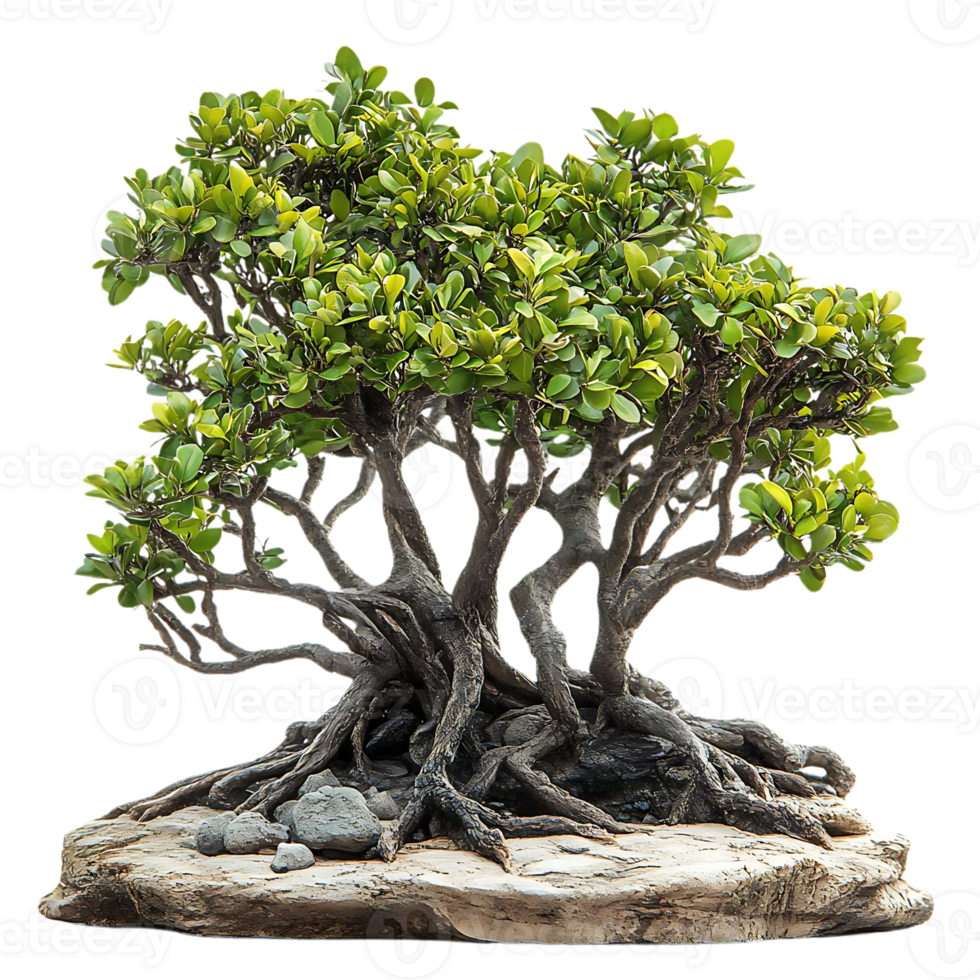
\includegraphics[width=0.7\columnwidth]{res/filler_b.png}
\end{center}
\columnbreak


